\section{Wakanda}
\label{ch:wakanda}

\subsection{Introduction}

Wakanda est une plateforme Open Source qui propose une dual licence, avec des capacités de développement strictement identique dans les deux cas. La création d'une communauté d’utilisateurs et contributeurs est clairement l’ambition première affichée par l’éditeur de Wakanda, dans le but de garantir la pérennité des projets et de s’adapter au foisonnement d’idées, de frameworks, d’appareils et d’usages qui se déroule sous nos yeux.


 
\begin{center}
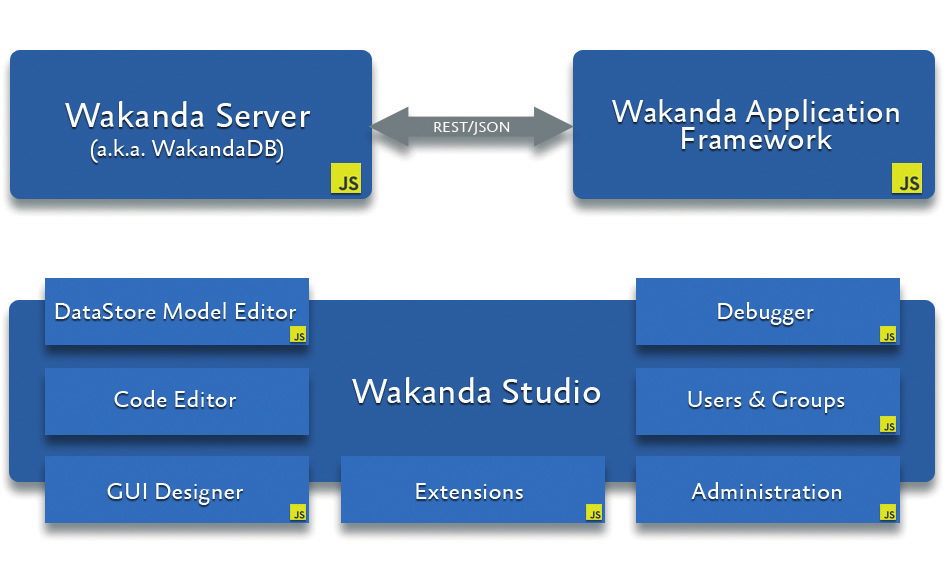
\includegraphics[scale=0.4]{img/wakanda.png}
\label{Plateforme Wakanda}
\end{center}




Au coeur de la plateforme se niche WakandaDBn un datastore objet NoSQL ultra-performant, qui, joint au moteur d’exécution JavaScript, basé sur Webkit, et à un serveur HTTP communiquant via JSON/REST constitue Wakanda Server, le back-end multi-plateformes (Linux, Mac, Windows) qui permettra d’héberger une solution Wakanda sur un serveur dédié, sur un Cloud privé ou public, en mode SaaS, etc...

Le framework Wakanda est automatiquement déployé vers les clients HTML et embarque un Data Provider qui se comporte comme un proxy des différentes DataClasses générées coté serveur. Ainsi de façon transparente, tous les objets JavaScript générés à l’aide du modèle de données sont exploitables via les différents widgets fournis avec le framework, mais également au travers de requêtes REST pour potentiellement connecter tout type d’interface, par ligne de commande ou à l’aide d’adaptateurs que pourront fournir des tierces parties, la communauté, ou l’éditeur 4D lui-même.
Enfin, le studio Wakanda vient compléter la suite de développement en proposant un IDE dédié capable de contrôler, via une application Desktop Mac ou Windows, aussi bien le modèle, les widgets, et l’adaptation cross-device de chaque écran coté client. Le studio fait la part belle à la gestion graphique du projet, et fait en sorte d’économiser à chaque étape l’écriture de code «technique». Le développeur peut dès lors se concentrer sur ses propres scripts et méthodes qui contiendront l’intelligence métier qui fera la valeur de son application. Outre les différents éditeurs (modèles, code, UI, utilisateurs et groupes) le studio propose une fenêtre d’administration des solutions et projets et un débuggeur qui permet de tracer le code JavaScript tournant sur le serveur. L’installation, tout comme le déploiement, s’effectuent par drag-and- drop d’un package sans aucune configuration. L’hébergement d’une solution Wakanda peut s’effectuer sur un serveur dédié, sur un VPS (serveur dédié virtuel, ou même sur une plateforme IaaS Cloud comme Amazon EC2 ou Rackspace. Côté mobile, Wakanda permet de réaliser des applications Web ou Hybrides, c’est-à-dire embarquées dans un runtime natif généré par PhoneGap. Il est également possible de créer des applications mobiles natives et d’accéder au Serveur via ses API REST et JSON-RPC.
